\documentclass[aps,pra,twocolumn,amsmath,amssymb,nofootinbib,superscriptaddress]{revtex4}

\newcommand{\bra}[1]{\langle#1|}
\newcommand{\ket}[1]{|#1\rangle}
\newcommand{\op}[2]{\hat{\textbf{#1}}_{#2}}
\newcommand{\dagop}[2]{\hat{\textbf{#1}}_{#2}^\dag}
\usepackage[pdftex]{graphicx}
\usepackage{mathrsfs}
\usepackage[colorlinks]{hyperref}

\begin{document}

\bibliographystyle{apsrev}

%
% Title
%

\title{QuantCoin\texttrademark\,-- A quantum computation-backed cryptocurrency}

%
% Authors
%

\author{Peter P. Rohde}
\email[]{dr.rohde@gmail.com}
\homepage{http://www.peterrohde.org}
\affiliation{Centre for Quantum Computation and Intelligent Systems (QCIS), Faculty of Engineering \& Information Technology, University of Technology Sydney, NSW 2007, Australia}

\date{\today}

\frenchspacing

%
% Abstract
%

\begin{abstract}
\end{abstract}

\maketitle

The Bitcoin mining process involves finding bit-strings that hash under SHA256\index{SHA256} to a value within some relatively small range. This so-called `proof-of-work' principle associates computational complexity with the mining process, and since the hashing functions are one-way functions, they must be evaluated via brute-force trial-and-error to find hits.

However, what a waste this is! Our proof-of-work is nothing more than hashing a huge number of random bit-strings, computations which are of no intrinsic value to anyone. The market value in turn has nothing to do with any inherent value earned during the mining process. Rather it is based purely on the psychology of scarcity, since there is an upper bound on the number of Bitcoins that satisfy the legitimacy constraint.

What if we were to replace brute-force hashing of random data with computations of genuine monetary value? Then we would have a sounder currency, whose value derives from the monetary cost of executing useful computations. While it is not so easy to invent such a protocol for classical computation, the idea lends itself very naturally to quantum computation, owing to their ability to undergo encrypted computation and be subject to verification protocols.

Building upon some of the pricing models introduced earlier in this section, there are two main candidates for backing a cryptocurrency with quantum compute-time: the spot market (i.e we execute the computation immediately); and the futures market (i.e we own the right to utilise the computer at some fixed time in the future). We consider the merits of both these candidates.

%
% Spot Market Model
%

\subsubsection{Spot market model}\index{Spot market}

In Alg.~\ref{alg:quant_coin} we provide a very rough sketch for how a protocol based on the spot market might be constructed. A corresponding graphical flowchart is shown in Fig.~\ref{fig:quantcoin_protocol}. We present the ideas in a very high-level manner, abstracting away the physical implementation details of the computation, encryption, and verification protocols, instead envisaging that we can interface with them using a very high-level API\index{API}.

\begin{table}[!htb]
\fbox{\parbox{0.965\columnwidth}{\texttt{ 
function QuantCoin($\hat{U}_\text{comp}$, blockchain, data, reward):
\begin{enumerate}
	\item Alice homomorphically/blindly encrypts $data$,
		\begin{align}
			encryptedInput = homoEncrypt(data)
		\end{align}
	\item Alice commits the $encryptedInput$ to the public $blockchain$,
	\begin{align}
	blockchain.commit(encryptedInput)	
	\end{align}
	\item Alice places into escrow Bob's $reward$,
	\begin{align}
		escrow.hold(reward)
	\end{align}
	\item Bob processes the $encryptedInput$ using $\hat{U}_\text{comp}$,
	\begin{align}
		encryptedOutput = \hat{U}_\text{comp}(encryptedInput)
	\end{align}
	\item Bob commits encrypted output to the $blockchain$,
	\begin{align}
	blockchain.commit(encryptedOutput)	
	\end{align}
	\item Alice and Bob execute a verification protocol,
	\begin{align}
	proof = verify(encryptedOutput)	
	\end{align}
	\item The $proof$ is committed to the $blockchain$ (as is every step of the proof if it is an interactive one),
	\begin{align}
		blockchain.commit(proof)
	\end{align}
	\item The $blockchain$ network inspects that the verification is valid.
	\item If valid, the $blockchain$ cryptographically hashes the data and proof, encapsulating it into a QuantCoin\texttrademark\,token, which is given to Bob,
	\begin{align}
		&token = SHA256(encryptedInput\nonumber\\
		&+ encryptedOutput + proof)\nonumber\\
		&Bob.receive(token)
	\end{align}
	\item The $reward$ held in escrow is released to Bob,
	\begin{align}
		escrow.release(Bob)
	\end{align}
\end{enumerate}}}}
\caption{Sketch for how a quantum computation-backed cryptocurrency might be implemented. We have abstracted away the underlying Blockchain protocol, interfacing with it using a high-level API, since Blockchain technology is highly liable to evolve. We similarly call upon verification subroutines using a high-level implementation-independent API.} \label{alg:quant_coin}
\end{table}

\begin{figure}[!htb]
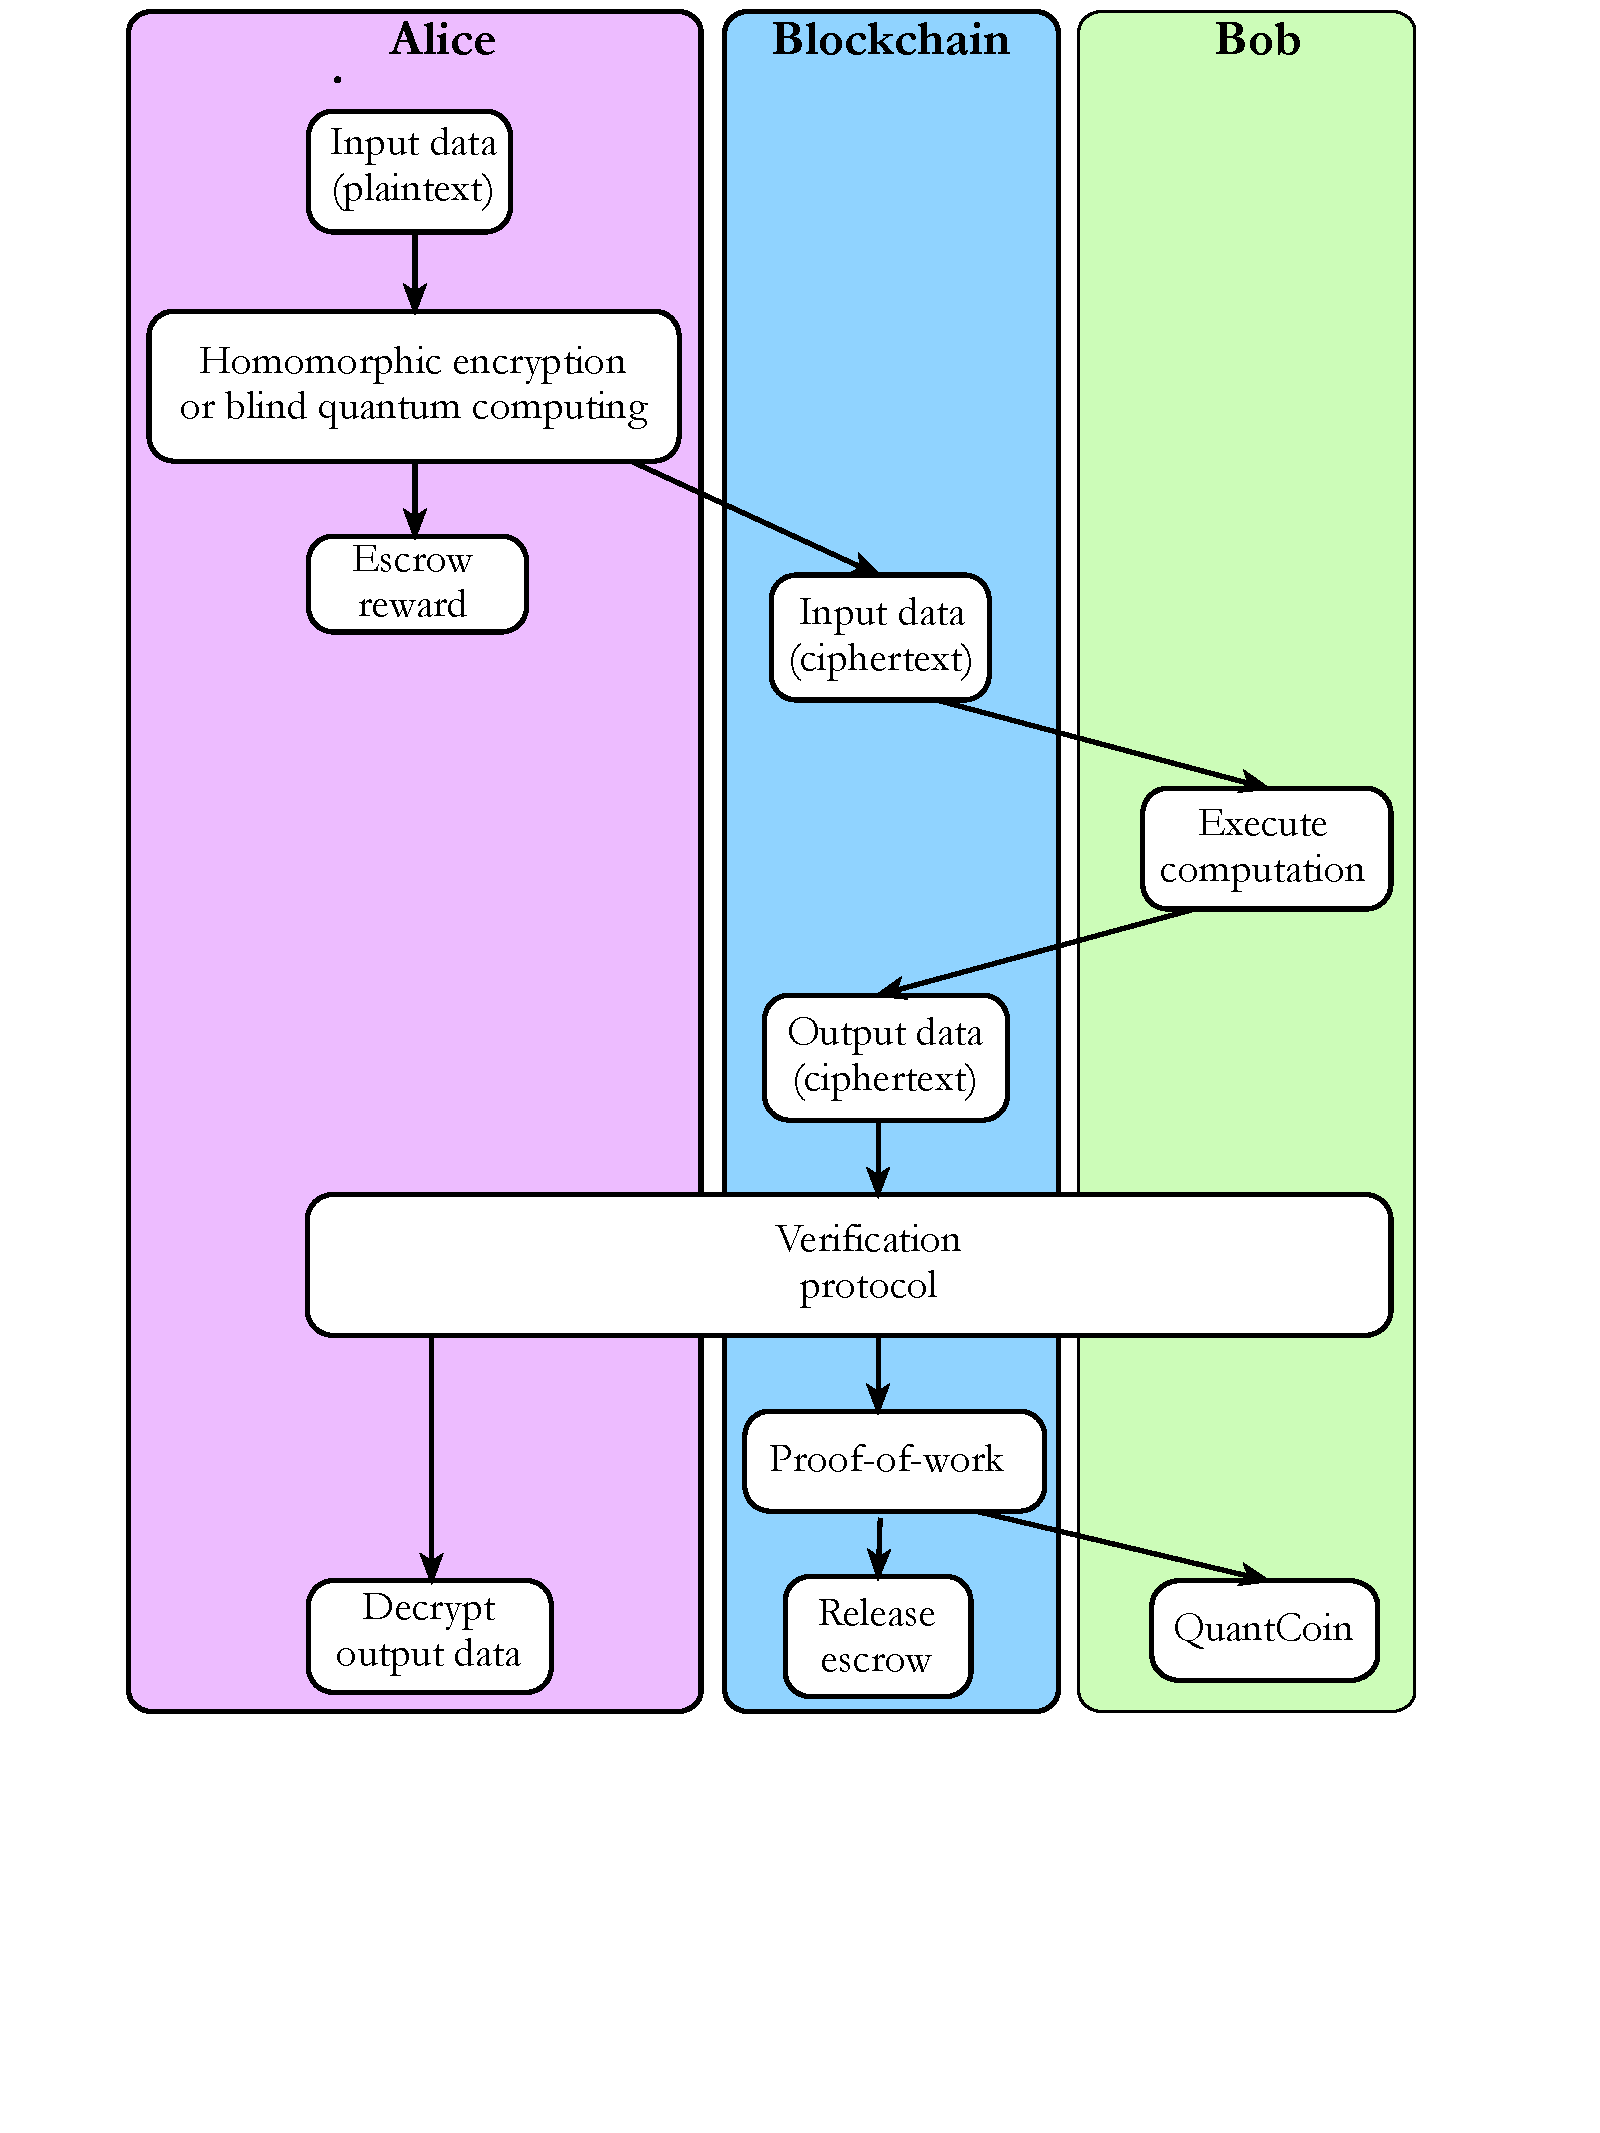
\includegraphics[width=0.47\textwidth]{quantcoin_protocol}
\caption{Flowchart for the QuantCoin\texttrademark\, protocol, introduced in Alg.~\ref{alg:quant_coin}.}\label{fig:quantcoin_protocol}	
\end{figure}

It is evident from the flow of Alg.~\ref{alg:quant_coin} that the mining process now comprises solving an actual quantum computation of intrinsic value to Alice, since she is exchanging assets (e.g dollars or already-existing QuantCoins\texttrademark) in exchange for the computation. Completion of the computation followed by successful verification then further rewards Bob with a fresh QuantCoin\texttrademark\, courtesy of the distributed Blockchain algorithm.

The described protocol, in addition to mining a new coin, associated with the execution of a computation, acts as a currency converter for converting traditional assets (e.g dollars) into QuantCoins\texttrademark. This ability to currency convert is necessary, and completely differs from the original Bitcoin mining process, where coins are fabricated out of thin air by anyone and everyone, independent of their pre-existing monetary wealth -- Bitcoins are not created via conversion from any existing asset. The fact that the computation associated with each QuantCoin\texttrademark\, is of intrinsic value on the other hand, implies that Alice ought to be paying something for the service.

Note that we observe an expansion in the money supply with each successfully executed and verified computation -- one additional unit of QuantCoins\texttrademark\, is mined for every unit of computation implemented. Unlike Bitcoin, there is no inherent theoretical upper limit on the number of coins that can exist. However the QuantCoin\texttrademark\, money supply\index{Money supply} will be limited for the practical reason that mining each one is associated with a monetary transaction between Alice and Bob, and Alice will eventually run out of assets to exchange for computations.

What relationships characterise the value of QuantCoins\texttrademark? First, in a perfectly efficient market (Sec.~\ref{sec:eff_markets}) we have,
\begin{align}\label{eq:value_quantcoins}
	&(\text{Dollar value of a QuantCoin\texttrademark\,}) \nonumber\\
	&+ (\text{Dollar value of reward paid by Alice for execution}) \nonumber\\
	&= (\text{Dollar value of cost of execution for Bob}).
\end{align}
 
Alternately, rather than Alice paying Bob's reward in dollars, she might pay for them in already-existing QuantCoins\texttrademark. Suppose Alice pays $\lambda$ QuantCoins\texttrademark\, as Bob's reward. Then Eq.~(\ref{eq:value_quantcoins}) reduces to,
\begin{align}
&(\text{Dollar value of a QuantCoin\texttrademark\,)}\\
&=\frac{1}{\lambda+1}(\text{Dollar value of cost of execution for Bob}),\nonumber
\end{align}
providing us with a simple financial model relating the market price of QuantCoins\texttrademark\, and the monetary cost of execution of computations.

Note that with exception to the scenario where Alice buys into QuantCoins\texttrademark\, using dollar currency (or any non-electronic asset that cannot be committed to the Blockchain), the entire protocol is self-enforcing via Blockchain transactions. Bob doesn't get paid his newly earned and freshly printed QuantCoin\texttrademark\, until the verification of the computation has completed and the proof committed to the Blockchain. He therefore cannot get paid until he has executed the computation he promised to, and proven to the network that he actually did.

The main security risk is that of Bob taking Alice's dollars and running, upon receiving the upfront reward in dollars, which necessarily don't reside on the Blockchain since they are not crypto-assets. This could be addressed by introducing trusted third-party escrow agents into the protocol. 

However, if the upfront payment were being made in pre-existing QuantCoins\texttrademark\,, the Blockchain might be programmed to not release the reward until completion of the final verification stage of the protocol -- effectively an escrow programmed directly into the Blockchain for self-execution.

%
% Futures Market Model
%

\subsubsection{Futures market model}

As described above, the cryptocurrency is effectively backed by the spot market in computation -- we exchange currency for the execution of computations \textit{immediately}. However, one might also envisage more complex cryptocurrencies being backed by the futures market in the licensing of quantum compute-time.

Intuitively, one would expect such a form of cryptocurrency to be sounder than the one backed by the spot market. This is because our spot market-derived coins, once mined are not guaranteed to be convertible to anything of value, including computations. Recall that the execution of the computation takes place immediately when the coin is created.

On the other hand, a QuantCoin\texttrademark\, backed by a guarantee to access quantum compute-time at a designated point in the future necessarily has value, so long as the demand for compute-time does, and maintains value until the contract matures and converts into compute-time at which point it becomes worthless.

\end{document}
